\section{Identification}
\label{sec:identification}

In order to control the system, we need to identify its parameters.

To do so, different tests type will be performed, such as:

\begin{enumerate}
    \item Direct measurement: measure all the quantity of the system that can be directly measured or retrieved from well established literature;
    \item Sensors characterization: create the mapping between the position of the ball and the output voltage of the infrared sensor and study the variance of all the sensors used internally in the control unit;
    \item Control to voltage: observe the relation between the control signal and the effective voltage applied to the coils;
    \item Inductances characterization: identify all the parameters needed to characterize inductances, based on the model proposed in Equation \ref{eq:model_for_inductance};
    \item Force validation: measure the force applied to the ball by the inductance in order to validate both the model and the parameters identified in the previous tests.
\end{enumerate}

Except for the first test, all the others will be performed leveraging the data acquisition system included in the \texttt{Inteco} control unit.

\subsection{Direct measurement}
\label{subsec:direct_measurement}

Many of the parameters of the system can be directly measured using a scale, a caliper or a voltmeter.

Among those, we have the mass of the ball $m$, the radius of the ball $r$, the distance between the upper and lower coils $h$ and the resistance of the coil $R$.
Their values are reported in Table \ref{tab:directly_measured_parameters}.

\begin{table}[H]

    \centering
    \begin{tabular}{|c|c|c|}
        \hline
        \textbf{Parameter} & \textbf{Value} & \textbf{Units} \\
        \hline
        $g$                & $9.81$         & $m/s^2$        \\
        $m$                & $0.06157$      & $kg$           \\
        $r$                & $0.06125/2$    & $m$            \\
        $h$                & $0.098$        & $m$            \\
        $R_{0}$            & $4.17$         & $\Omega$       \\
        \hline
    \end{tabular}

    \caption{Directly measured parameters and constants}
    \label{tab:directly_measured_parameters}

\end{table}
\subsection{Sensors characterization}
\label{subsec:sensors_characterization}

In this subsection, we will focus on the characterization of the sensors used internally by the control unit to measure or estimate the system state.



\subsubsection{Voltage to position mapping}
\label{subsubsec:voltage_to_position}

At first, we need to create the mapping between the voltage output of the infrared sensor and the position of the ball.
To do so, we simply sample the output voltage of the infrared sensor and the position of the ball using the data acquisition system included in the \texttt{Inteco} control unit and a caliper.

The obtained data is shown in Figure \ref{fig:voltage_to_position}.

\begin{figure}[H]
    \centering
    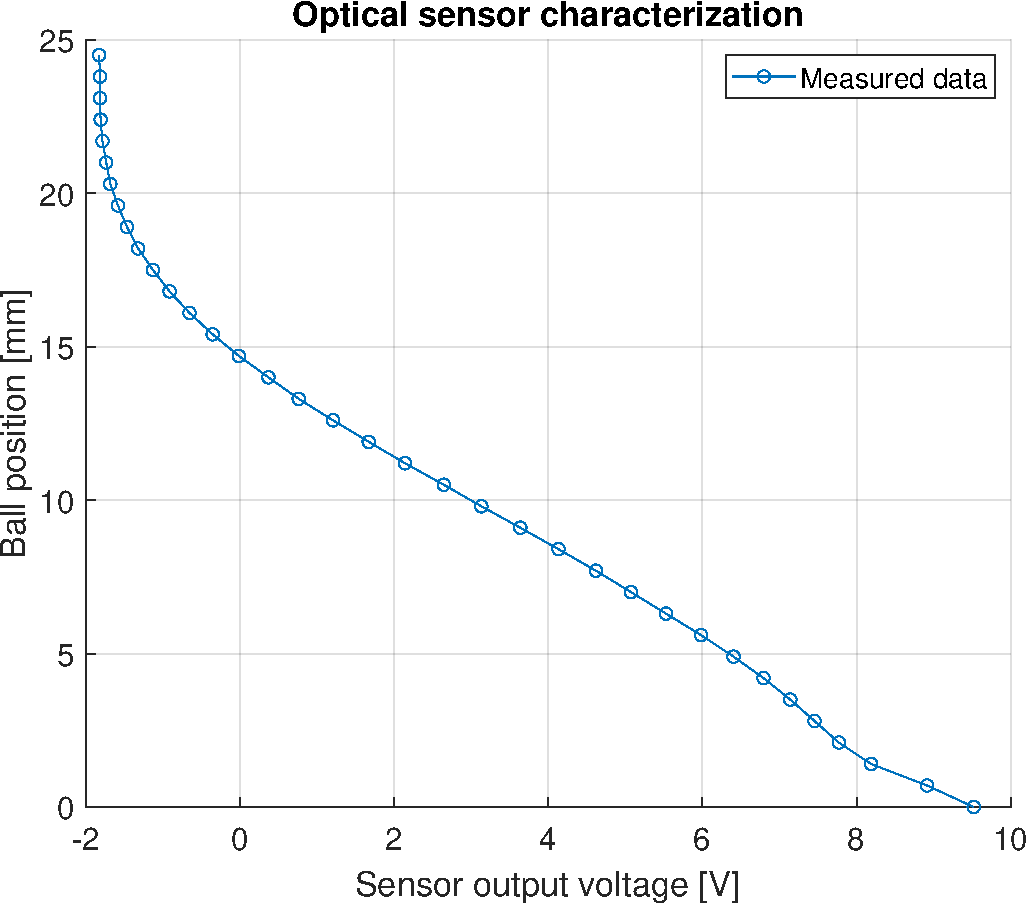
\includegraphics[width=0.6\textwidth]{img/MATLAB/identification/sensor_position.pdf}
    \caption{Position of the ball as a function of the output voltage of the infrared optical sensor.}
    \label{fig:voltage_to_position}
\end{figure}

One can clearly see the non-linear relationship between the ball's position and the output voltage of the infrared sensor.

Moreover, it's important to underline the hardware limitations of the sensor that allows a maximum measurement distance of $\approx 20 [mm]$ from the upper coil before reaching its saturation limit.



\subsubsection{Sensors noise analysis}
\label{subsubsec:sensors_noise}

A comprehensive analysis of the sensors' noise is crucial to correctly estimate both the position of the ball and the coils' current.
The experimental setup consists of keeping the ball at a fixed position and recording the sensors' output for a certain amount of time imposing a zero control signal.
The analysis then assumes the sensors' noise to be a zero-mean Gaussian white noise process.

With this optics, we can estimate the standard deviation for each sensor and use it to design the filters and estimators in the following sections (see Section \ref{sec:filters_estimators_design}).

\begin{figure}[H]
    \centering
    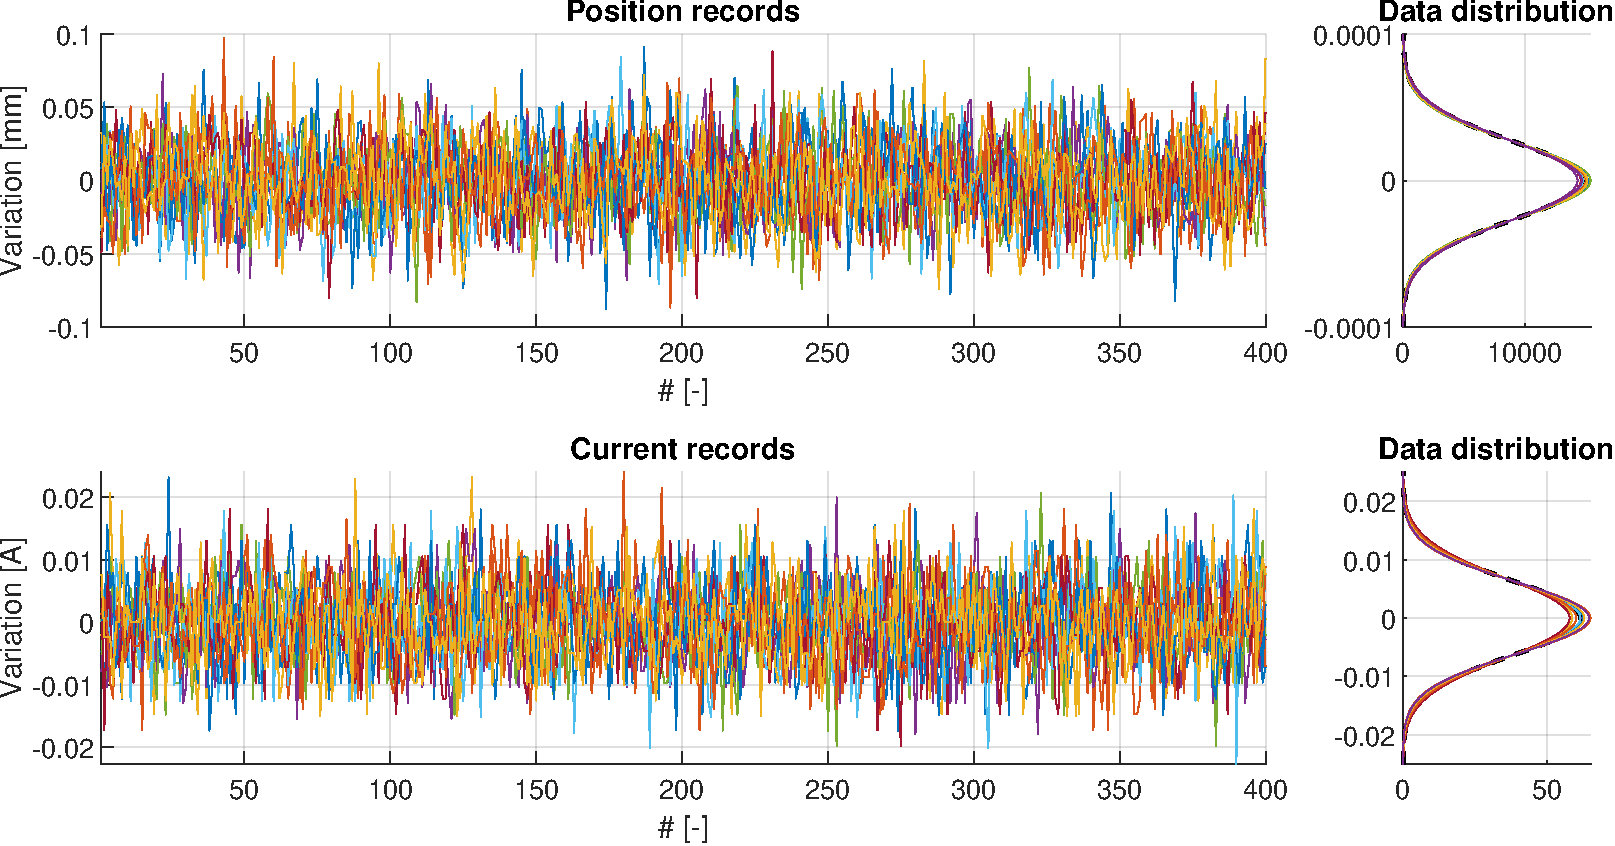
\includegraphics[width=1\textwidth]{img/MATLAB/identification/sensor_noises.pdf}
    \caption{Sensors' noise analysis. \hl{Repeat the test inside the infrared sensor saturation limit.}}
    \label{fig:sensors_noise}
\end{figure}

In Figure \ref{fig:sensors_noise}, the analysis of the sensors' noise is shown.

The left plots show the time history of the sensor output variations, while the right plots show the Gaussian distribution of the sensors' noise with the mean distribution marked with a dashed black line.
The upper plots refer to the infrared sensor, while the lower plots refer to the current sensor.

The standard deviation and covariance of the sensors' noise is reported in Table \ref{tab:sensors_noise}.

\begin{table}[H]
    \centering

    \begin{tabular}{|c|c|c|}
        \hline
        \textbf{Sensor} & \textbf{Standard deviation}        & \textbf{Covariance}                  \\
        \hline
        Infrared        & $1.402804 \cdot 10^{-3} \quad [m]$ & $7.166031 \cdot 10^{-6} \quad [m^2]$ \\
        Current         & $6.327979 \cdot 10^{-3} \quad [A]$ & $4.005490 \cdot 10^{-5} \quad [A^2]$ \\
        \hline
    \end{tabular}

    \caption{Standard deviation and covariance of the sensors' noise.}
    \label{tab:sensors_noise}

\end{table}

\subsection{Control to voltage}
\label{subsec:control_to_voltage}

As said in the previous section of mathematical modeling, we need to identify the relation between the control signal and the effective voltage applied to the coils.
The control unit provided by \texttt{Inteco} it's programmed to receive a PWM duty cycle as input and to convert it into a voltage that is applied to the coils.
In order to identify this relation, we simply apply many duty cycles to the control unit and measure the corresponding voltage applied to the coils using a multimeter.

The output of this test is a series of points that can be fitted to a linear model having an initial black zone where the control action is not effective on the voltage applied to the coils.
In Figure \ref{fig:control_to_voltage} we can observe both the measured points, the linear fitting and the effective voltage applied considering the black zone.

\begin{figure}[H]
    \centering
    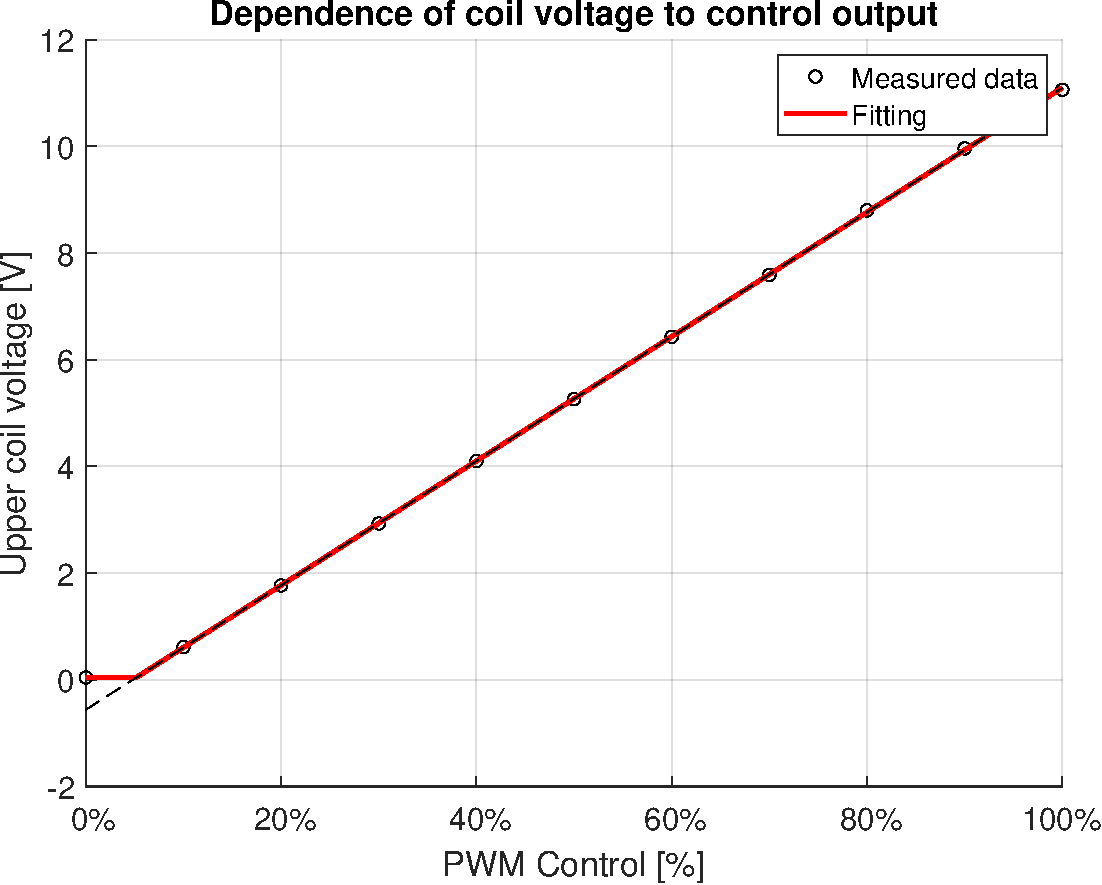
\includegraphics[width=0.6\textwidth]{img/MATLAB/identification/control_to_voltage.pdf}
    \caption{Control to voltage identification}
    \label{fig:control_to_voltage}
\end{figure}

As we can see, the linear model for the relation $V_* = f(U) = f(\text{PWM})$ is a good approximation outside the initial black zone control.
Because of this, we can consider the following control to voltage relation:

\begin{equation}
    V_* = \begin{cases}
        V_{*min}    & \text{if } U < U_{min}    \\
        k_* U + c_* & \text{if } U \geq U_{min}
    \end{cases}
\end{equation}

Where $V_{*min}$ is the minimum voltage applied to the coils when the control signal is zero, $u_{min}$ is the minimum control signal that is effective on the voltage applied to the coils, $k_*$ is the slope of the linear model and $c_*$ is the offset of the linear model.

The values of the parameters are shown in Table \ref{tab:control_to_voltage_parameters}.

\begin{table}[H]

    \centering
    \begin{tabular}{|c|c|c|}
        \hline
        \textbf{Parameter} & \textbf{Value}            & \textbf{Units} \\
        \hline
        $V_{*min}$         & $4.300000 \cdot 10^{-2}$  & $V$            \\
        $U_{min}$          & $5.179276$                & $\%$           \\
        $k_*$              & $1.165800 \cdot 10^{1}$   & $V/\%$         \\
        $c_*$              & $-5.608000 \cdot 10^{-1}$ & $V$            \\
        \hline
    \end{tabular}

    \caption{Control to voltage identification parameters}
    \label{tab:control_to_voltage_parameters}

\end{table}
\subsection{Inductances characterization}
\label{subsec:inductances_characterization}

A key parameter of the system is the inductance of the coils.

As already proposed in Equation \ref{eq:model_for_inductance}, the inductance of the coils cannot be considered constant and both its dependence on the current and the position of the ball must be taken into account when dealing with the \acrshort{mls}.

In order to identify the inductance of the coils and all the parameters needed to characterize them, we have to measure $L(z, I)$ for many currents and ball positions.
Once these values are known, we can fit the data to the model proposed in Equation \ref{eq:model_for_inductance} and identify its parameters.

Given a certain (fix in time) position of the ball and a certain current step input, we can measure the value of the inductance of the coils, knowing that:

\begin{equation}
    V = R I + \frac{d (L I)}{d t} = R I + \left( \frac{\partial L}{\partial I} I + L \right) \dot{I}
\end{equation}

If we suppose for a moment that the variation of the inductance with the current is negligible, we can obtain a closed form solution for the current in the RL circuit as follows:

\begin{equation}
    I(t) = \frac{V_{final}}{R_0} \left( 1 - e^{- \frac{R_0}{L} t} \right)
    \label{eq:current_in_rl_circuit}
\end{equation}

Given the previous equations, we can adopt the following strategy to fully characterize the inductance of the coils over the range of possible ball positions and currents:

\begin{enumerate}
    \item Fix the ball at a certain height ($z^*$);
    \item Apply a certain current step input to the system ($I^*$);
    \item Measure the current in the coils ($I(t)$);
    \item Fit the measured current to the model proposed in Equation \ref{eq:current_in_rl_circuit} and identify $L(z^*, I^*)$;
    \item Repeat from step 2 for different step inputs of currents;
    \item Repeat from step 1 for different ball positions.
\end{enumerate}

In Figure \ref{fig:inductance_characterization_currents} we can see on the left all the experimental data representing the dynamics of the current in the coils for different step inputs of currents and different ball positions, while on the right we can see the fitting of some experimental data to the model proposed in Equation \ref{eq:current_in_rl_circuit}.

\begin{figure}[H]
    \centering
    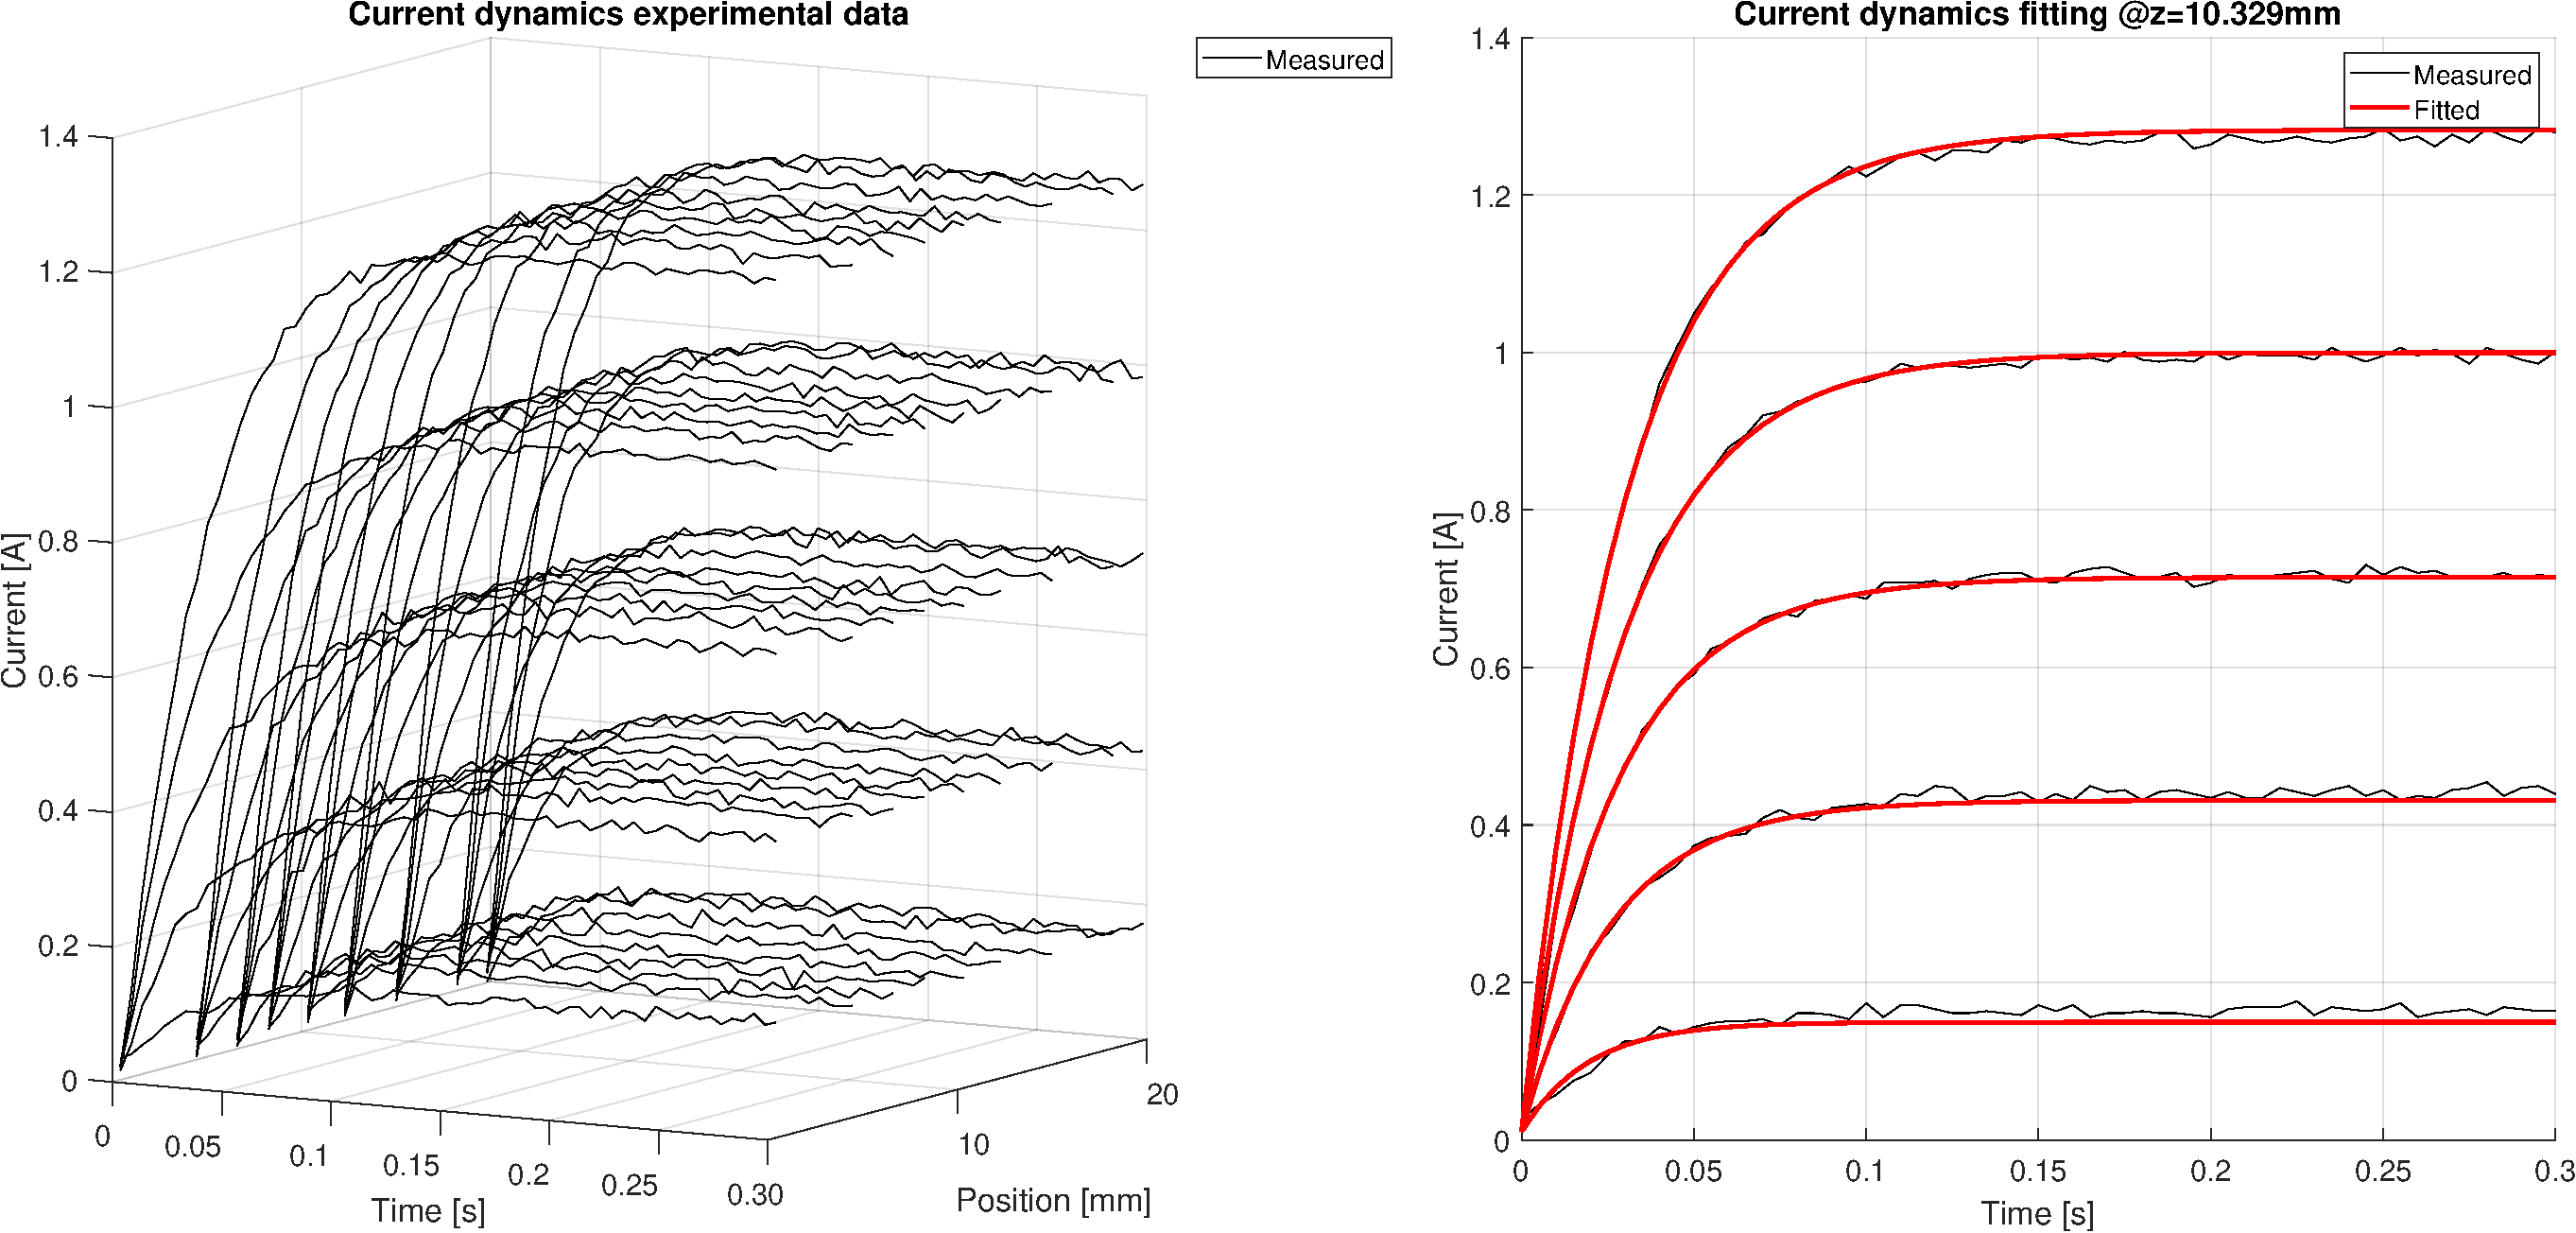
\includegraphics[width=1\textwidth]{img/MATLAB/identification/currents.pdf}
    \caption{Inductance characterization for different currents and ball positions}
    \label{fig:inductance_characterization_currents}
\end{figure}

From the right side of Figure \ref{fig:inductance_characterization_currents} we can see that the fitting of the data to the model proposed in Equation \ref{eq:current_in_rl_circuit} is optimal for middle values of the current, while it tends to underestimate and overestimate the current for low and high values of the current, respectively.
This behavior is probably due to the fact that the variation of the inductance with the current that has been neglected in the model of the current (Equation \ref{eq:current_in_rl_circuit}) is not negligible and should have been taken into account.

Thanks to the data obtained from the multiple tests, we can now fit the values of the inductance of the coils to the model proposed in Equation \ref{eq:model_for_inductance} and identify its parameters.
The obtained model fitting is shown in Figure \ref{fig:inductance_characterization_inductance}.

\begin{figure}[H]
    \centering
    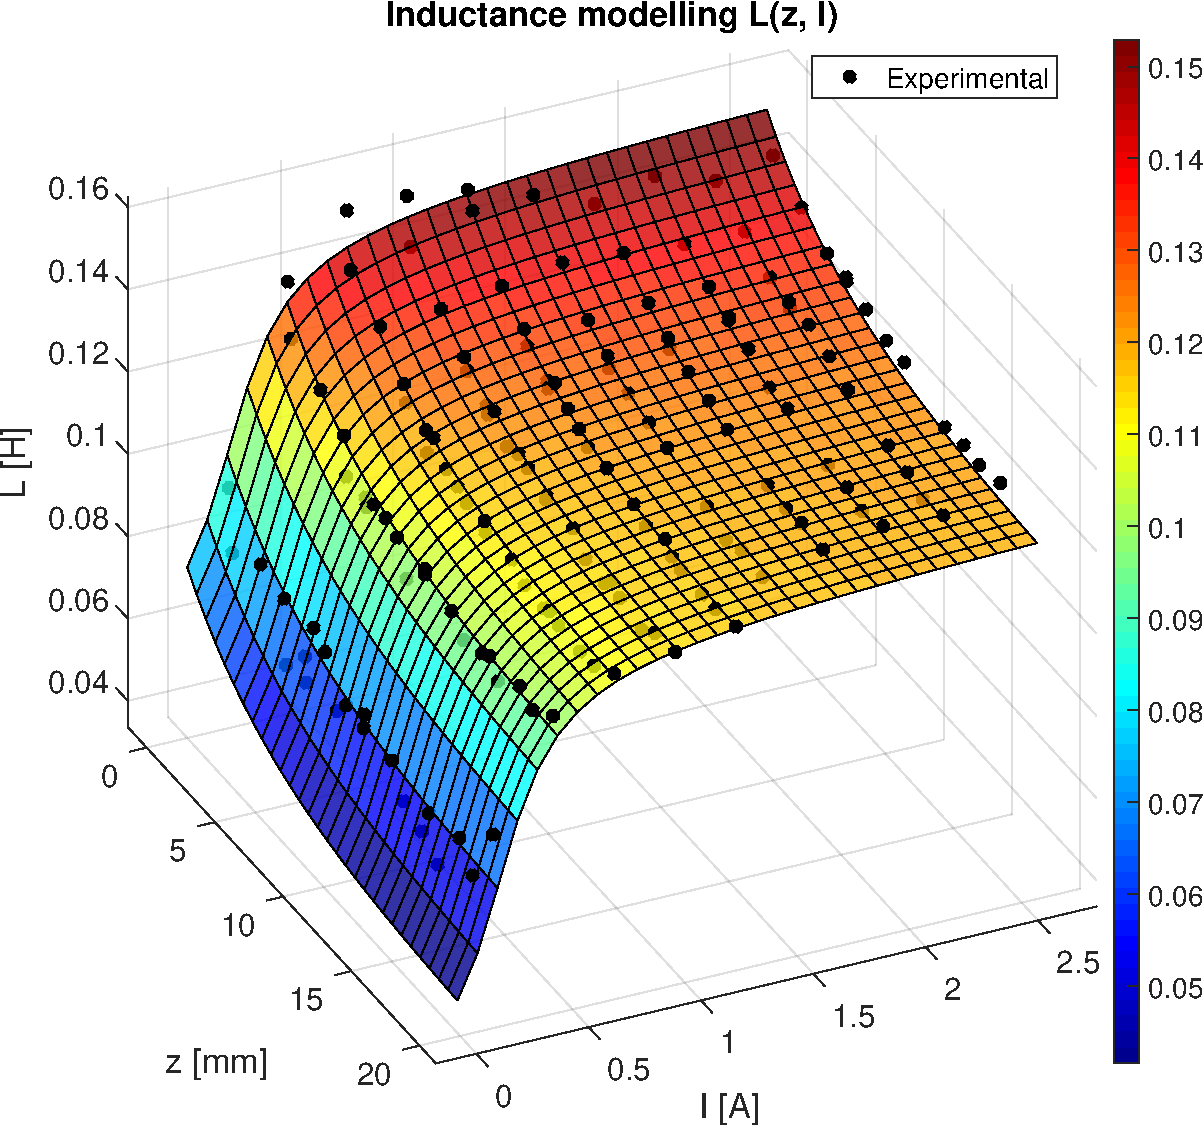
\includegraphics[width=0.6\textwidth]{img/MATLAB/identification/inductance.pdf}
    \caption{Inductance model fitting}
    \label{fig:inductance_characterization_inductance}
\end{figure}

The $210$ black dots in Figure \ref{fig:inductance_characterization_inductance} represent the experimental data obtained from the fitting of currents dynamics for different current steps and ball positions.

The values of the parameters are shown in Table \ref{tab:inductance_characterization_parameters}.

\begin{table}[H]
    \centering
    \begin{tabular}{|c|c|c|}
        \hline
        \textbf{Parameter} & \textbf{Value}           & \textbf{Units} \\
        \hline
        $L_0$              & $6.122809 \cdot 10^{-2}$ & $H$            \\
        $a_z$              & $1.837302 \cdot 10^{+2}$ & $1/m$          \\
        $L_z$              & $3.438228 \cdot 10^{-2}$ & $H$            \\
        $a_I$              & $4.759750 \cdot 10^{+0}$ &                \\
        $b_I$              & $6.704755 \cdot 10^{-1}$ & $A$            \\
        $L_I$              & $3.831209 \cdot 10^{-2}$ & $H$            \\
        \hline
    \end{tabular}

    \caption{Inductance characterization parameters}
    \label{tab:inductance_characterization_parameters}

\end{table}

As a double check against the model proposed in Equation \ref{eq:model_for_inductance}, one can also observe the R squared value of the fitting $R^2 = 0.961$, which is a good indicator of the quality of the fitting.

\subsection{Force validation}
\label{subsec:force_validation}

Finally, we can proceed with the force validation test.

Thanks to the data obtained from the previous tests, we are already able to predict the force applied to the ball by the inductance.
In particular, we already know that the electromagnetic force applied to the ball is given by the following equation:

\begin{equation}
    F_{em} = \frac{1}{2} \frac{\partial L}{\partial z} I^2 = \frac{1}{2} (-a_z L_z e^{-a_z z}) I^2
\end{equation}

Because of the previously identified parameters, we have an analytical expression for the sensitivity of the inductance with respect to the position of the ball.
However, due to uncertainties in the identification of the parameters, we can expect some discrepancies between the predicted force and the measured one.

In order to quantify these discrepancies and validate the model, we use a direct method to measure the force applied to the ball by the inductance and compare it with the predicted one.
To do so, we recall Equation \ref{eq:reduced_equations_of_motion_final} and in particular the equation relative to $\dot{v}$:

\begin{equation}
    \dot{v} = m^{-1} \left(\frac{1}{2} \frac{\partial L_1}{\partial z} I_1^2 + \frac{1}{2} \frac{\partial L_2}{\partial z} I_2^2 + m g  \right)
\end{equation}

If we consider the system at rest or equivalently at the incipient motion of the ball, we can simplify the equation as follows:

\begin{equation}
    0 = \frac{1}{2} \frac{\partial L_1}{\partial z} I_1^2 + \frac{1}{2} \frac{\partial L_2}{\partial z} I_2^2 + m g
\end{equation}

Supposing now that only the first coil is energized, we can further simplify the equation as follows:

\begin{equation}
    0 = \frac{1}{2} \frac{\partial L_1}{\partial z} I_1^2 + m g
\end{equation}

Which leads to:

\begin{equation}
    \frac{\partial L_1}{\partial z} = -2 \frac{m g}{I_1^2}
    \label{eq:sensitivity_of_inductance}
\end{equation}

This last equation basically tells us that in steady state conditions, when the ball is levitating (i.e. $\dot{z} = 0$ and not supported by any platform), the sensitivity of the inductance of the first coil has an analytical expression that can be directly evaluated by measuring the current in the first coil and the position of the ball.

In order to follow this approach, the experimental steps are as follows:

\begin{enumerate}
    \item By regulating a lower platform, the ball is placed at a certain height ($z^*$);
    \item A linearly increasing voltage is applied to the first coil;
    \item The current circulating in the first coil is measured;
    \item The current at which the ball starts to levitate is identified;
    \item The sensitivity of the inductance is calculated using Equation \ref{eq:sensitivity_of_inductance}.
    \item The test is repeated for different initial positions of the ball.
\end{enumerate}

In Figure \ref{fig:levitation_current} we can see both the position of the ball (red line) and the current circulating in the first coil (black line) around the identified levitation point (marked by the vertical black dashed line).

\begin{figure}[H]
    \centering
    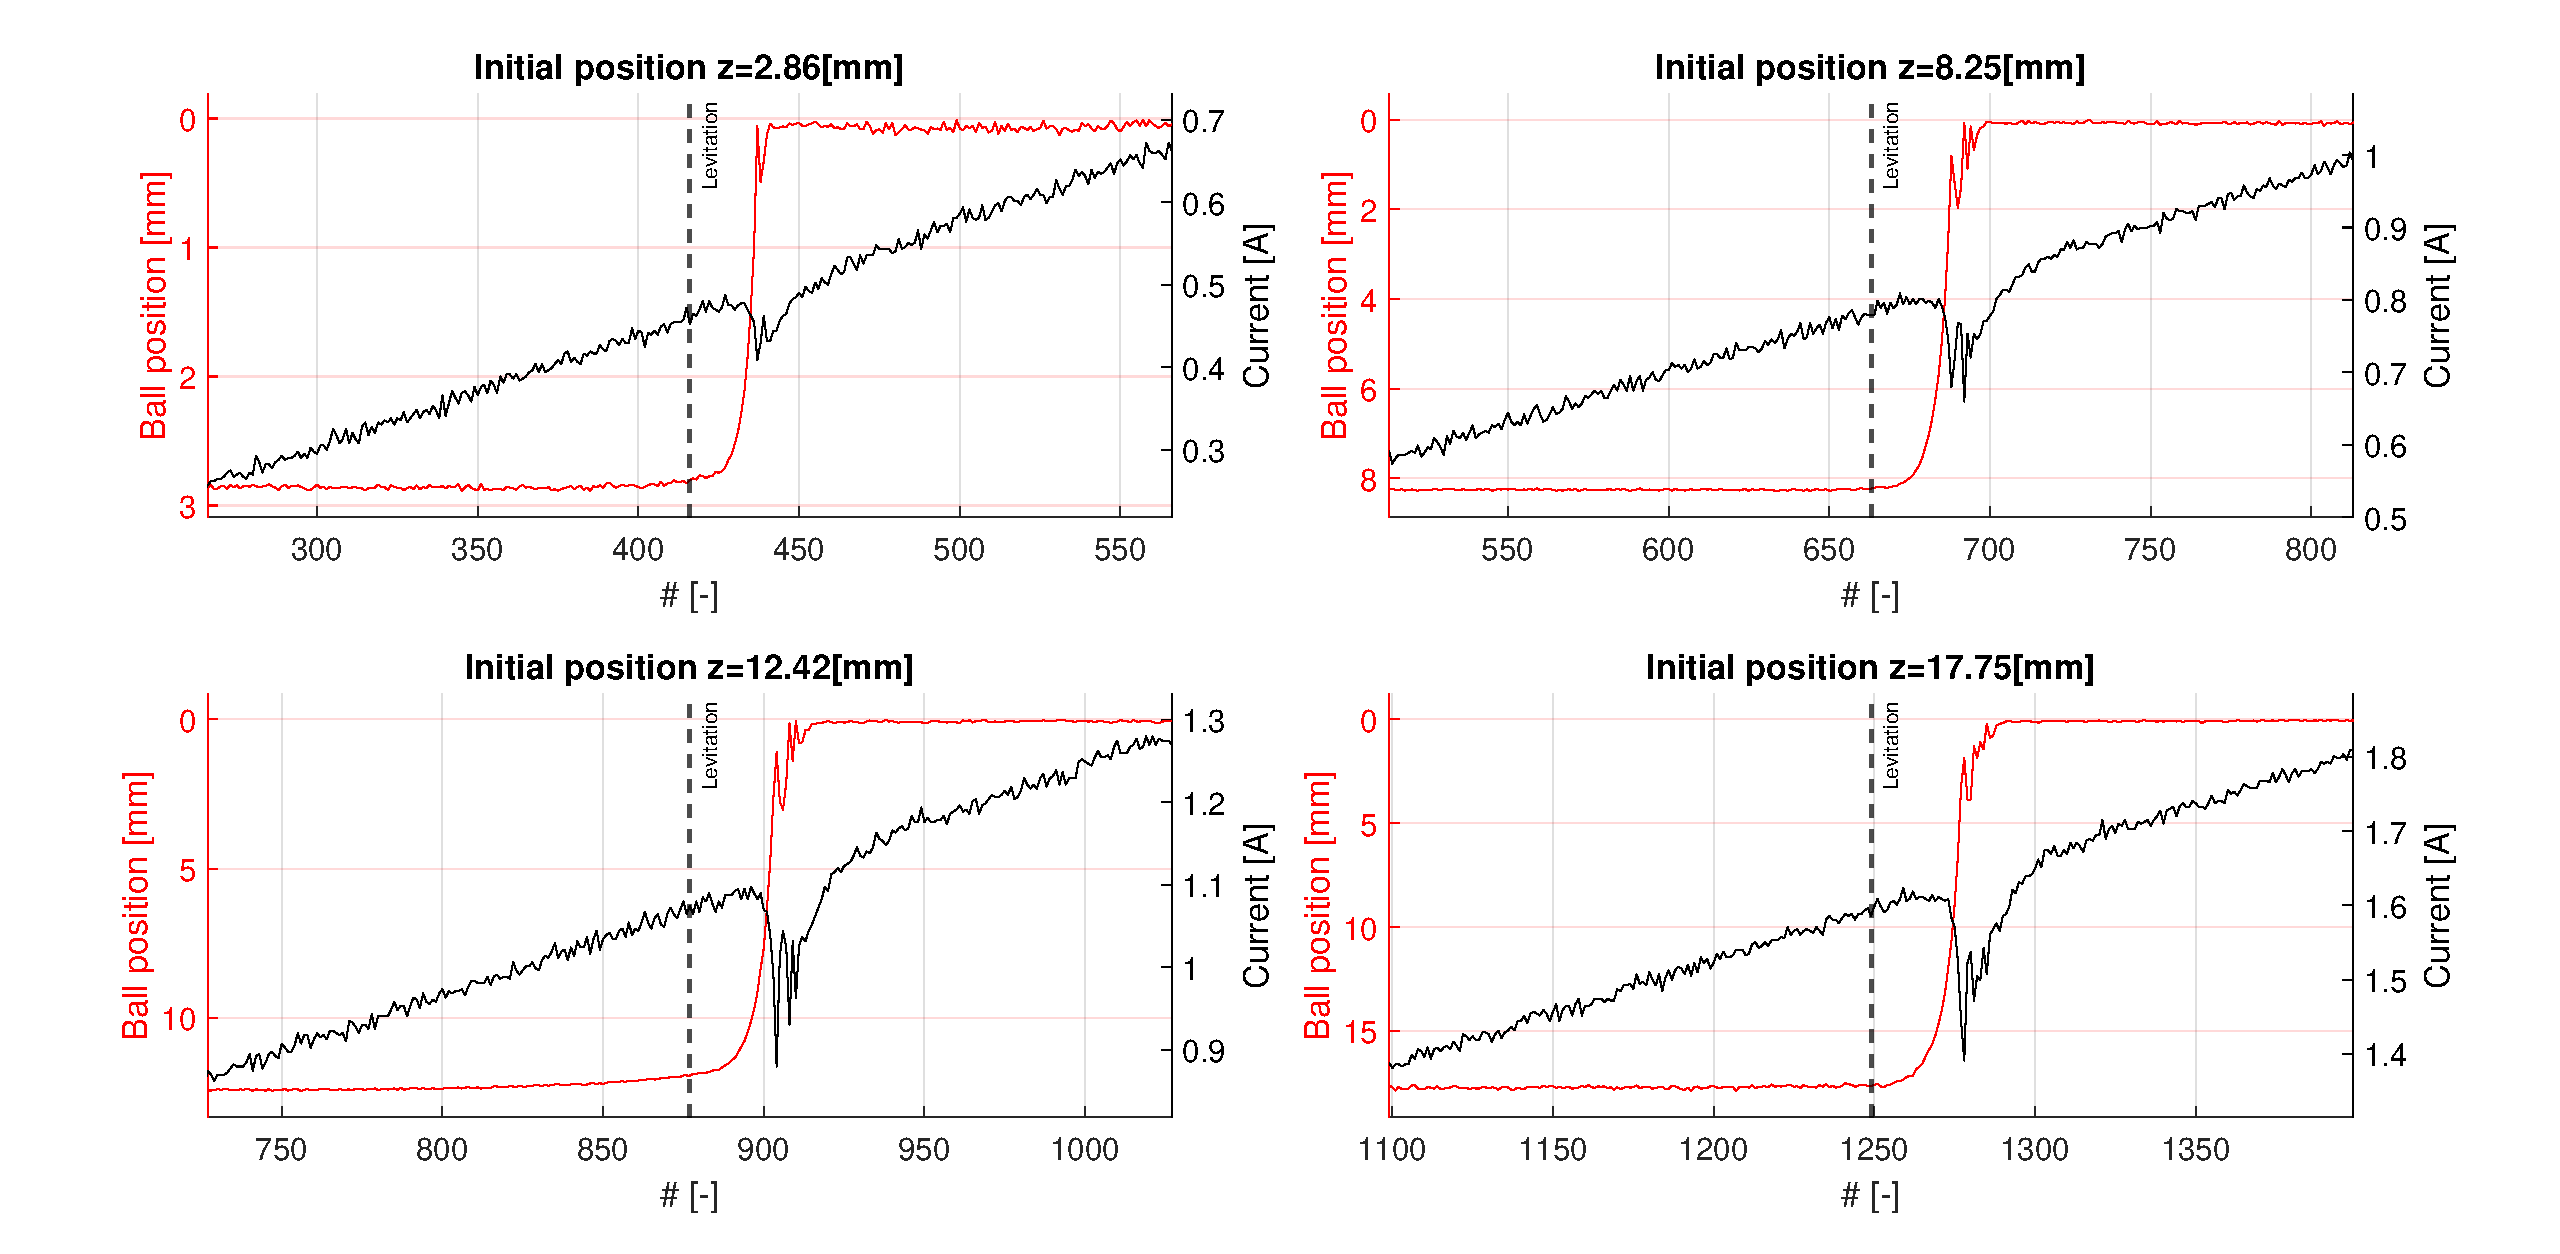
\includegraphics[width=1\textwidth]{img/MATLAB/identification/currents_for_force.pdf}
    \caption{Position of the ball and current in the first coil around the levitation point (marked by vertical black dashed line)}
    \label{fig:levitation_current}
\end{figure}

Instead, in Figure \ref{fig:dynamic_inductance_characteristics}, we can observe both the measured data and the fitted ones.
On the right side figure, a complete characterization of the electromagnetic force has been reconstructed based again on the above equations.

\begin{figure}[H]
    \centering
    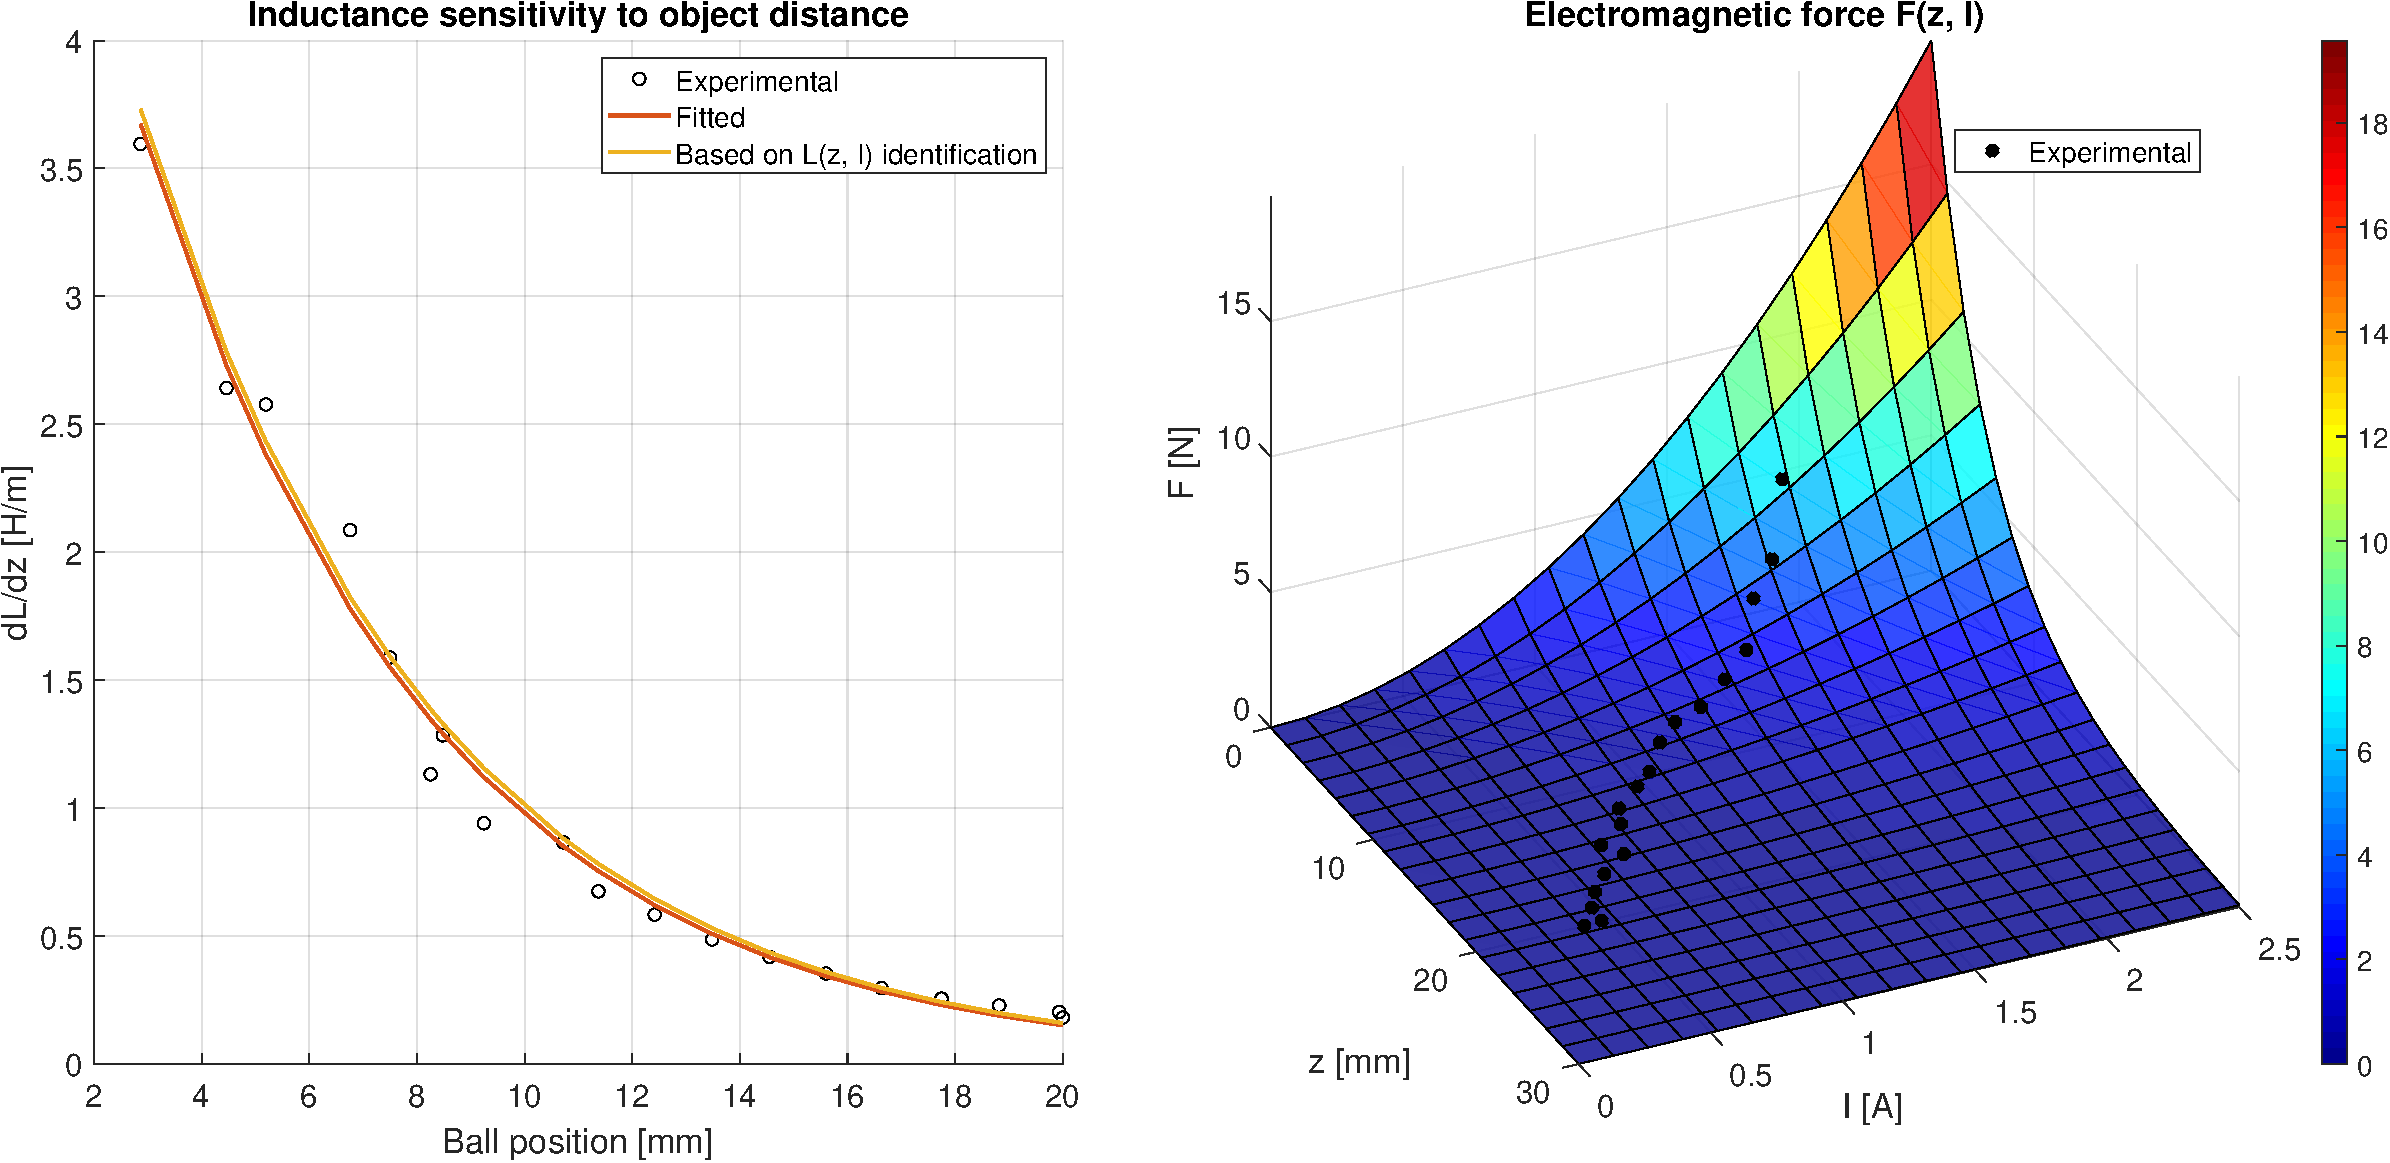
\includegraphics[width=1\textwidth]{img/MATLAB/identification/force.pdf}
    \caption{Dynamic inductance characteristics and electromagnet force}
    \label{fig:dynamic_inductance_characteristics}
\end{figure}

The left-hand side of Figure \ref{fig:dynamic_inductance_characteristics} shows a comparison between the measured data (black circles), their fitting (red line) and the sensitivity of the inductance coming from the parameters identified in Section \ref{subsec:inductances_characterization} (yellow line).
Data shows great accuracy in almost the entire range of the ball position.

The right-hand side of Figure \ref{fig:dynamic_inductance_characteristics} shows the electromagnetic force generated by the first coil as a function of both the ball position and the current circulating in the coil.
One can notice that the force has an exponential behavior with respect to the ball position and a quadratic behavior with respect to the current.